\begin{enumerate}[label=\thesection.\arabic*,ref=\thesection.\theenumi]
\numberwithin{equation}{enumi}
\numberwithin{figure}{enumi}
\numberwithin{table}{enumi}
\item In the Figure \ref{fig:9/9/2/1}, $ABCD$ is a parallelogram, $AE \perp DC$ and $CF \perp AD$. If $AB = 16 cm$, $AE = 8 cm$, and $CF = 10cm$, find $AD$.
	\begin{figure}[!h]
		\centering
 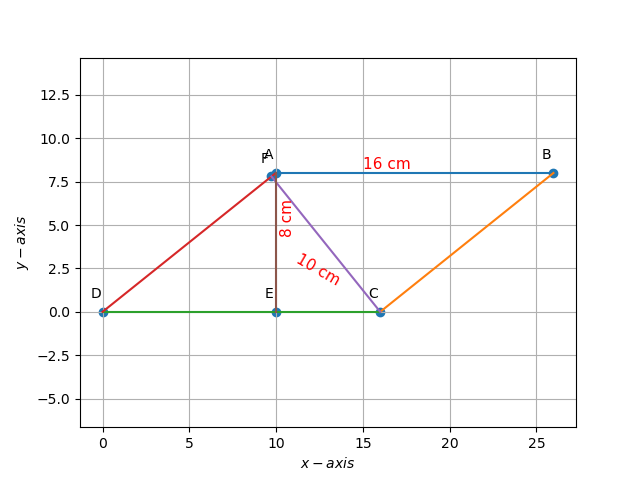
\includegraphics[width=\columnwidth]{chapters/9/9/2/1/figs/fig1.pdf}
		\caption{}
		\label{fig:9/9/2/1}
  	\end{figure}
%\documentclass[12pt]{article}
%\usepackage[cmex10]{amsmath}
%\usepackage{amsthm}
%\usepackage{mathrsfs}
%\usepackage{txfonts}
%\usepackage{stfloats}
%\usepackage{bm}
%\usepackage{cite}
%\usepackage{cases}
%\usepackage{subfig}
%\usepackage{longtable}
%\usepackage{multirow}
%\usepackage{enumitem}
%\usepackage{mathtools}
%\usepackage{steinmetz}
%\usepackage{tikz}
%\usepackage{circuitikz}
%\usepackage{verbatim}
%\usepackage{tfrupee}
%\usepackage[breaklinks=true]{hyperref}
%\usepackage{tkz-euclide} % loads  TikZ and tkz-base
%\providecommand{\brak}[1]{\ensuremath{\left(#1\right)}}
%\usepackage{atbegshi}
%\AtBeginDocument{\AtBeginShipoutNext{\AtBeginShipoutDiscard}}
%\usetikzlibrary{calc,math}
%\usepackage{listings}
%    \usepackage{color}                                            %%
%    \usepackage{array}                                            %%
 %   \usepackage{longtable}                                        %%
  %  \usepackage{calc}                                             %%
   % \usepackage{multirow}                                         %%
    %\usepackage{hhline}                                           %%
    %\usepackage{ifthen}                                           %%
  %optionally (for landscape tables embedded in another document): %%
    %\usepackage{lscape}     
%\usepackage{multicol}
%\usepackage{chngcntr}

%\DeclareMathOperator*{\Res}{Res}
%\renewcommand{\baselinestretch}{2}
%\renewcommand\thesection{\arabic{section}}
%\renewcommand\thesubsection{\thesection.\arabic{subsection}}
%\renewcommand\thesubsubsection{\thesubsection.\arabic{subsubsection}}


% correct bad hyphenation here
%\hyphenation{op-tical net-works semi-conduc-tor}
%\def\inputGnumericTable{}                                 %%

%\lstset{
%language=C,
%frame=single, 
%breaklines=true,
%columns=fullflexible
%}
%\begin{document}
%\newtheorem{theorem}{Theorem}[section]
%\newtheorem{problem}{Problem}
%\newtheorem{proposition}{Proposition}[section]
%\newtheorem{lemma}{Lemma}[section]
%\newtheorem{corollary}[theorem]{Corollary}
%\newtheorem{example}{Example}[section]
%\newtheorem{definition}[problem]{Definition}
%\newcommand{\BEQA}{\begin{eqnarray}}
%\newcommand{\EEQA}{\end{eqnarray}}
%\newcommand{\define}{\stackrel{\triangle}{=}}

%\bibliographystyle{IEEEtran}
%\bibliographystyle{ieeetr}
%\providecommand{\mbf}{\mathbf}
%\providecommand{\pr}[1]{\ensuremath{\Pr\left(#1\right)}}
%\providecommand{\qfunc}[1]{\ensuremath{Q\left(#1\right)}}
%\providecommand{\sbrak}[1]{\ensuremath{{}\left[#1\right]}}
%\providecommand{\lsbrak}[1]{\ensuremath{{}\left[#1\right.}}
%\providecommand{\rsbrak}[1]{\ensuremath{{}\left.#1\right]}}
%\providecommand{\brak}[1]{\ensuremath{\left(#1\right)}}
%\providecommand{\lbrak}[1]{\ensuremath{\left(#1\right.}}
%\providecommand{\rbrak}[1]{\ensuremath{\left.#1\right)}}
%\providecommand{\cbrak}[1]{\ensuremath{\left\{#1\right\}}}
%\providecommand{\lcbrak}[1]{\ensuremath{\left\{#1\right.}}
%\providecommand{\rcbrak}[1]{\ensuremath{\left.#1\right\}}}
%\theoremstyle{remark}
%\newtheorem{rem}{Remark}
%\newcommand{\sgn}{\mathop{\mathrm{sgn}}}
%\providecommand{\res}[1]{\Res\displaylimits_{#1}} 
%\providecommand{\mtx}[1]{\mathbf{#1}}
%\providecommand{\fourier}{\overset{\mathcal{F}}{\rightleftharpoons}}
%\providecommand{\system}{\overset{\mathcal{H}}{\longleftrightarrow}}
	%\newcommand{\solution}[2]{\textbf{Solution:}{#1}}
%\newcommand{\solution}{\noindent \textbf{Solution: }}
%\newcommand{\cosec}{\,\text{cosec}\,}
%\providecommand{\dec}[2]{\ensuremath{\overset{#1}{\underset{#2}{\gtrless}}}}
%\newcommand{\myvec}[1]{\ensuremath{\begin{pmatrix}#1\end{pmatrix}}}
%\newcommand{\mydet}[1]{\ensuremath{\begin{vmatrix}#1\end{vmatrix}}}
%\let\vec\mathbf
%\begin{center}
%\title{\textbf{Straight Lines}}
%\date{\vspace{-5ex}} %Not to print date automatically
%\maketitle
%\end{center}
%\setcounter{page}{1}
%\section*{11$^{th}$ Maths - Chapter 10}
%This is Problem-10 from Exercise 10.4
%\begin{enumerate}
%    \item If three lines whose equations are $y=m_1x+c_1$, $y=m_2x+c_2$ and $y=m_3x+c_3$ are concurrent, then show that $m_1(c_2-c_3)+m_2(c_3-c_1)+m_3(c_1-c_2) = 0.$\\
%    \solution 
    Given lines can be written as \begin{align}
       m_1x-y+c_1=0
    \end{align}
    \begin{align}
        m_2x-y+c_2=0
    \end{align}
    \begin{align}
        m_3x-y+c_3=0
        \label{eq:3}
    \end{align}
    
    
   The above lines can be written in the form of \begin{align}
        \Vec{n}^{\top}\Vec{x} = c
    \end{align}
   Therefore,
		\begin{align}
       \myvec{m_1&-1}\vec{x}=c_1
       \label{eq:5}
   \end{align} 
   \begin{align}
       \myvec{m_2&-1}\vec{x}=c_2
       \label{eq:6}
   \end{align}
   \begin{align}
       \myvec{m_3&-1}\vec{x}=c_3
       \label{eq:7}
   \end{align}
   Solving equations \eqref{eq:5}, \eqref{eq:6}and \eqref{eq:7}
		augumented matrix is
 \begin{align}
    \myvec{m_1&-1&c_1\\m_2&-1&c_2\\m_3&-1&c_3}\\
    \xleftrightarrow{R_2 \leftarrow m_1R_2-m_2R_1}
    \myvec{m_1&-1&c_1\\0&m_2-m_1&m_1c_2-m_2c_1\\m_3&-1&c_3}\\
    \xleftrightarrow{R_3 \leftarrow m_1R_3-m_3R_1}
    \myvec{m_1&-1&c_1\\0&m_2-m_1&m_1c_2-m_2c_1\\0&m_3-m_1&m_1c_3-m_3c_1}\\
    \xleftrightarrow{R_3 \leftarrow R_3\frac{m_2-m_1}{m_3-m_1}-R_2}
        \myvec{m_1&-1&c_1\\0&m_2-m_1&m_1c_2-m_2c_1\\0&0&$\brak{m_1c_3-m_3c_1}$$\brak{\frac{m_2-m_1}{m_3-m_1}}$-$\brak{m_1c_2-m_2c_1}$}
\end{align}
Now, for lines to be concurrent, then the third row should be equal to zero. \\

Therefore,
\begin{align}
\brak{m_1c_3-m_3c_1}\brak{\frac{m_2-m_1}{m_3-m_1}}-\brak{m_1c_2-m_2c_1}=0\\
\frac{\brak{m_1c_3-m_3c_1}\brak{m_2-m_1}-\brak{m_1c_2-m_2c_1}\brak{m_3-m_1}}{m_3-m_1}=0\\
\brak{m_1c_3-m_3c_1}\brak{m_2-m_1}-\brak{m_1c_2-m_2c_1}\brak{m_3-m_1}=0\\
m_2c_3-m_1c_3+m_3c_1-m_3c_2+m_1c_2-m_2c_1=0\\
m_1\brak{c_2-c_3}+m_2\brak{c_3-c_1}+m_3\brak{c_1-c_2} = 0
\end{align}
           Hence proved
%\begin{figure}[h]
 %   \centering
  %  \includegraphics[width=\columnwidth]{concurrent-1.png}
   % \caption{Straight Lines}
    %\label{fig:concurrent-1.png}
%\end{figure}
%\end{enumerate}
%\end{document}

\item For a given Parallelogram $ABCD$, show that for any
point $\vec{P}$ inside the parallelogram,
\begin{enumerate}
	\item $Ar(APD)+Ar(PBC) = \frac{1}{2}Ar(ABCD)$
	\item $Ar(APD)+Ar(PBC) = Ar(APB)+Ar(PCD)$
\end{enumerate}
%\documentclass[12pt]{article}
%\usepackage[cmex10]{amsmath}
%\usepackage{amsthm}
%\usepackage{mathrsfs}
%\usepackage{txfonts}
%\usepackage{stfloats}
%\usepackage{bm}
%\usepackage{cite}
%\usepackage{cases}
%\usepackage{subfig}
%\usepackage{longtable}
%\usepackage{multirow}
%\usepackage{enumitem}
%\usepackage{mathtools}
%\usepackage{steinmetz}
%\usepackage{tikz}
%\usepackage{circuitikz}
%\usepackage{verbatim}
%\usepackage{tfrupee}
%\usepackage[breaklinks=true]{hyperref}
%\usepackage{tkz-euclide} % loads  TikZ and tkz-base
%\providecommand{\brak}[1]{\ensuremath{\left(#1\right)}}
%\usepackage{atbegshi}
%\AtBeginDocument{\AtBeginShipoutNext{\AtBeginShipoutDiscard}}
%\usetikzlibrary{calc,math}
%\usepackage{listings}
%    \usepackage{color}                                            %%
%    \usepackage{array}                                            %%
 %   \usepackage{longtable}                                        %%
  %  \usepackage{calc}                                             %%
   % \usepackage{multirow}                                         %%
    %\usepackage{hhline}                                           %%
    %\usepackage{ifthen}                                           %%
  %optionally (for landscape tables embedded in another document): %%
    %\usepackage{lscape}     
%\usepackage{multicol}
%\usepackage{chngcntr}

%\DeclareMathOperator*{\Res}{Res}
%\renewcommand{\baselinestretch}{2}
%\renewcommand\thesection{\arabic{section}}
%\renewcommand\thesubsection{\thesection.\arabic{subsection}}
%\renewcommand\thesubsubsection{\thesubsection.\arabic{subsubsection}}


% correct bad hyphenation here
%\hyphenation{op-tical net-works semi-conduc-tor}
%\def\inputGnumericTable{}                                 %%

%\lstset{
%language=C,
%frame=single, 
%breaklines=true,
%columns=fullflexible
%}
%\begin{document}
%\newtheorem{theorem}{Theorem}[section]
%\newtheorem{problem}{Problem}
%\newtheorem{proposition}{Proposition}[section]
%\newtheorem{lemma}{Lemma}[section]
%\newtheorem{corollary}[theorem]{Corollary}
%\newtheorem{example}{Example}[section]
%\newtheorem{definition}[problem]{Definition}
%\newcommand{\BEQA}{\begin{eqnarray}}
%\newcommand{\EEQA}{\end{eqnarray}}
%\newcommand{\define}{\stackrel{\triangle}{=}}

%\bibliographystyle{IEEEtran}
%\bibliographystyle{ieeetr}
%\providecommand{\mbf}{\mathbf}
%\providecommand{\pr}[1]{\ensuremath{\Pr\left(#1\right)}}
%\providecommand{\qfunc}[1]{\ensuremath{Q\left(#1\right)}}
%\providecommand{\sbrak}[1]{\ensuremath{{}\left[#1\right]}}
%\providecommand{\lsbrak}[1]{\ensuremath{{}\left[#1\right.}}
%\providecommand{\rsbrak}[1]{\ensuremath{{}\left.#1\right]}}
%\providecommand{\brak}[1]{\ensuremath{\left(#1\right)}}
%\providecommand{\lbrak}[1]{\ensuremath{\left(#1\right.}}
%\providecommand{\rbrak}[1]{\ensuremath{\left.#1\right)}}
%\providecommand{\cbrak}[1]{\ensuremath{\left\{#1\right\}}}
%\providecommand{\lcbrak}[1]{\ensuremath{\left\{#1\right.}}
%\providecommand{\rcbrak}[1]{\ensuremath{\left.#1\right\}}}
%\theoremstyle{remark}
%\newtheorem{rem}{Remark}
%\newcommand{\sgn}{\mathop{\mathrm{sgn}}}
%\providecommand{\res}[1]{\Res\displaylimits_{#1}} 
%\providecommand{\mtx}[1]{\mathbf{#1}}
%\providecommand{\fourier}{\overset{\mathcal{F}}{\rightleftharpoons}}
%\providecommand{\system}{\overset{\mathcal{H}}{\longleftrightarrow}}
	%\newcommand{\solution}[2]{\textbf{Solution:}{#1}}
%\newcommand{\solution}{\noindent \textbf{Solution: }}
%\newcommand{\cosec}{\,\text{cosec}\,}
%\providecommand{\dec}[2]{\ensuremath{\overset{#1}{\underset{#2}{\gtrless}}}}
%\newcommand{\myvec}[1]{\ensuremath{\begin{pmatrix}#1\end{pmatrix}}}
%\newcommand{\mydet}[1]{\ensuremath{\begin{vmatrix}#1\end{vmatrix}}}
%\let\vec\mathbf
%\begin{center}
%\title{\textbf{Straight Lines}}
%\date{\vspace{-5ex}} %Not to print date automatically
%\maketitle
%\end{center}
%\setcounter{page}{1}
%\section*{11$^{th}$ Maths - Chapter 10}
%This is Problem-10 from Exercise 10.4
%\begin{enumerate}
%    \item If three lines whose equations are $y=m_1x+c_1$, $y=m_2x+c_2$ and $y=m_3x+c_3$ are concurrent, then show that $m_1(c_2-c_3)+m_2(c_3-c_1)+m_3(c_1-c_2) = 0.$\\
%    \solution 
    Given lines can be written as \begin{align}
       m_1x-y+c_1=0
    \end{align}
    \begin{align}
        m_2x-y+c_2=0
    \end{align}
    \begin{align}
        m_3x-y+c_3=0
        \label{eq:3}
    \end{align}
    
    
   The above lines can be written in the form of \begin{align}
        \Vec{n}^{\top}\Vec{x} = c
    \end{align}
   Therefore,
		\begin{align}
       \myvec{m_1&-1}\vec{x}=c_1
       \label{eq:5}
   \end{align} 
   \begin{align}
       \myvec{m_2&-1}\vec{x}=c_2
       \label{eq:6}
   \end{align}
   \begin{align}
       \myvec{m_3&-1}\vec{x}=c_3
       \label{eq:7}
   \end{align}
   Solving equations \eqref{eq:5}, \eqref{eq:6}and \eqref{eq:7}
		augumented matrix is
 \begin{align}
    \myvec{m_1&-1&c_1\\m_2&-1&c_2\\m_3&-1&c_3}\\
    \xleftrightarrow{R_2 \leftarrow m_1R_2-m_2R_1}
    \myvec{m_1&-1&c_1\\0&m_2-m_1&m_1c_2-m_2c_1\\m_3&-1&c_3}\\
    \xleftrightarrow{R_3 \leftarrow m_1R_3-m_3R_1}
    \myvec{m_1&-1&c_1\\0&m_2-m_1&m_1c_2-m_2c_1\\0&m_3-m_1&m_1c_3-m_3c_1}\\
    \xleftrightarrow{R_3 \leftarrow R_3\frac{m_2-m_1}{m_3-m_1}-R_2}
        \myvec{m_1&-1&c_1\\0&m_2-m_1&m_1c_2-m_2c_1\\0&0&$\brak{m_1c_3-m_3c_1}$$\brak{\frac{m_2-m_1}{m_3-m_1}}$-$\brak{m_1c_2-m_2c_1}$}
\end{align}
Now, for lines to be concurrent, then the third row should be equal to zero. \\

Therefore,
\begin{align}
\brak{m_1c_3-m_3c_1}\brak{\frac{m_2-m_1}{m_3-m_1}}-\brak{m_1c_2-m_2c_1}=0\\
\frac{\brak{m_1c_3-m_3c_1}\brak{m_2-m_1}-\brak{m_1c_2-m_2c_1}\brak{m_3-m_1}}{m_3-m_1}=0\\
\brak{m_1c_3-m_3c_1}\brak{m_2-m_1}-\brak{m_1c_2-m_2c_1}\brak{m_3-m_1}=0\\
m_2c_3-m_1c_3+m_3c_1-m_3c_2+m_1c_2-m_2c_1=0\\
m_1\brak{c_2-c_3}+m_2\brak{c_3-c_1}+m_3\brak{c_1-c_2} = 0
\end{align}
           Hence proved
%\begin{figure}[h]
 %   \centering
  %  \includegraphics[width=\columnwidth]{concurrent-1.png}
   % \caption{Straight Lines}
    %\label{fig:concurrent-1.png}
%\end{figure}
%\end{enumerate}
%\end{document}

\item In Fig.
		\ref{fig:9/9/2/5},
$PQRS$ and $ABRS$ are parallelograms
and $\vec{X}$ is any point on side $BR$. Show that  
\begin{enumerate}
    \item $ar (PQRS) = ar(ABRS)$
	    \label{prop:9/9/2/5}
    \item $ar(AXS) = \frac{1}{2} ar(PQRS)$
\end{enumerate}
	\begin{figure}[!h]
		\centering
 \includegraphics[width=\columnwidth]{chapters/9/9/2/5/figs/parallelogram1.pdf}
		\caption{}
		\label{fig:9/9/2/5}
  	\end{figure}
%\documentclass[12pt]{article}
%\usepackage[cmex10]{amsmath}
%\usepackage{amsthm}
%\usepackage{mathrsfs}
%\usepackage{txfonts}
%\usepackage{stfloats}
%\usepackage{bm}
%\usepackage{cite}
%\usepackage{cases}
%\usepackage{subfig}
%\usepackage{longtable}
%\usepackage{multirow}
%\usepackage{enumitem}
%\usepackage{mathtools}
%\usepackage{steinmetz}
%\usepackage{tikz}
%\usepackage{circuitikz}
%\usepackage{verbatim}
%\usepackage{tfrupee}
%\usepackage[breaklinks=true]{hyperref}
%\usepackage{tkz-euclide} % loads  TikZ and tkz-base
%\providecommand{\brak}[1]{\ensuremath{\left(#1\right)}}
%\usepackage{atbegshi}
%\AtBeginDocument{\AtBeginShipoutNext{\AtBeginShipoutDiscard}}
%\usetikzlibrary{calc,math}
%\usepackage{listings}
%    \usepackage{color}                                            %%
%    \usepackage{array}                                            %%
 %   \usepackage{longtable}                                        %%
  %  \usepackage{calc}                                             %%
   % \usepackage{multirow}                                         %%
    %\usepackage{hhline}                                           %%
    %\usepackage{ifthen}                                           %%
  %optionally (for landscape tables embedded in another document): %%
    %\usepackage{lscape}     
%\usepackage{multicol}
%\usepackage{chngcntr}

%\DeclareMathOperator*{\Res}{Res}
%\renewcommand{\baselinestretch}{2}
%\renewcommand\thesection{\arabic{section}}
%\renewcommand\thesubsection{\thesection.\arabic{subsection}}
%\renewcommand\thesubsubsection{\thesubsection.\arabic{subsubsection}}


% correct bad hyphenation here
%\hyphenation{op-tical net-works semi-conduc-tor}
%\def\inputGnumericTable{}                                 %%

%\lstset{
%language=C,
%frame=single, 
%breaklines=true,
%columns=fullflexible
%}
%\begin{document}
%\newtheorem{theorem}{Theorem}[section]
%\newtheorem{problem}{Problem}
%\newtheorem{proposition}{Proposition}[section]
%\newtheorem{lemma}{Lemma}[section]
%\newtheorem{corollary}[theorem]{Corollary}
%\newtheorem{example}{Example}[section]
%\newtheorem{definition}[problem]{Definition}
%\newcommand{\BEQA}{\begin{eqnarray}}
%\newcommand{\EEQA}{\end{eqnarray}}
%\newcommand{\define}{\stackrel{\triangle}{=}}

%\bibliographystyle{IEEEtran}
%\bibliographystyle{ieeetr}
%\providecommand{\mbf}{\mathbf}
%\providecommand{\pr}[1]{\ensuremath{\Pr\left(#1\right)}}
%\providecommand{\qfunc}[1]{\ensuremath{Q\left(#1\right)}}
%\providecommand{\sbrak}[1]{\ensuremath{{}\left[#1\right]}}
%\providecommand{\lsbrak}[1]{\ensuremath{{}\left[#1\right.}}
%\providecommand{\rsbrak}[1]{\ensuremath{{}\left.#1\right]}}
%\providecommand{\brak}[1]{\ensuremath{\left(#1\right)}}
%\providecommand{\lbrak}[1]{\ensuremath{\left(#1\right.}}
%\providecommand{\rbrak}[1]{\ensuremath{\left.#1\right)}}
%\providecommand{\cbrak}[1]{\ensuremath{\left\{#1\right\}}}
%\providecommand{\lcbrak}[1]{\ensuremath{\left\{#1\right.}}
%\providecommand{\rcbrak}[1]{\ensuremath{\left.#1\right\}}}
%\theoremstyle{remark}
%\newtheorem{rem}{Remark}
%\newcommand{\sgn}{\mathop{\mathrm{sgn}}}
%\providecommand{\res}[1]{\Res\displaylimits_{#1}} 
%\providecommand{\mtx}[1]{\mathbf{#1}}
%\providecommand{\fourier}{\overset{\mathcal{F}}{\rightleftharpoons}}
%\providecommand{\system}{\overset{\mathcal{H}}{\longleftrightarrow}}
	%\newcommand{\solution}[2]{\textbf{Solution:}{#1}}
%\newcommand{\solution}{\noindent \textbf{Solution: }}
%\newcommand{\cosec}{\,\text{cosec}\,}
%\providecommand{\dec}[2]{\ensuremath{\overset{#1}{\underset{#2}{\gtrless}}}}
%\newcommand{\myvec}[1]{\ensuremath{\begin{pmatrix}#1\end{pmatrix}}}
%\newcommand{\mydet}[1]{\ensuremath{\begin{vmatrix}#1\end{vmatrix}}}
%\let\vec\mathbf
%\begin{center}
%\title{\textbf{Straight Lines}}
%\date{\vspace{-5ex}} %Not to print date automatically
%\maketitle
%\end{center}
%\setcounter{page}{1}
%\section*{11$^{th}$ Maths - Chapter 10}
%This is Problem-10 from Exercise 10.4
%\begin{enumerate}
%    \item If three lines whose equations are $y=m_1x+c_1$, $y=m_2x+c_2$ and $y=m_3x+c_3$ are concurrent, then show that $m_1(c_2-c_3)+m_2(c_3-c_1)+m_3(c_1-c_2) = 0.$\\
%    \solution 
    Given lines can be written as \begin{align}
       m_1x-y+c_1=0
    \end{align}
    \begin{align}
        m_2x-y+c_2=0
    \end{align}
    \begin{align}
        m_3x-y+c_3=0
        \label{eq:3}
    \end{align}
    
    
   The above lines can be written in the form of \begin{align}
        \Vec{n}^{\top}\Vec{x} = c
    \end{align}
   Therefore,
		\begin{align}
       \myvec{m_1&-1}\vec{x}=c_1
       \label{eq:5}
   \end{align} 
   \begin{align}
       \myvec{m_2&-1}\vec{x}=c_2
       \label{eq:6}
   \end{align}
   \begin{align}
       \myvec{m_3&-1}\vec{x}=c_3
       \label{eq:7}
   \end{align}
   Solving equations \eqref{eq:5}, \eqref{eq:6}and \eqref{eq:7}
		augumented matrix is
 \begin{align}
    \myvec{m_1&-1&c_1\\m_2&-1&c_2\\m_3&-1&c_3}\\
    \xleftrightarrow{R_2 \leftarrow m_1R_2-m_2R_1}
    \myvec{m_1&-1&c_1\\0&m_2-m_1&m_1c_2-m_2c_1\\m_3&-1&c_3}\\
    \xleftrightarrow{R_3 \leftarrow m_1R_3-m_3R_1}
    \myvec{m_1&-1&c_1\\0&m_2-m_1&m_1c_2-m_2c_1\\0&m_3-m_1&m_1c_3-m_3c_1}\\
    \xleftrightarrow{R_3 \leftarrow R_3\frac{m_2-m_1}{m_3-m_1}-R_2}
        \myvec{m_1&-1&c_1\\0&m_2-m_1&m_1c_2-m_2c_1\\0&0&$\brak{m_1c_3-m_3c_1}$$\brak{\frac{m_2-m_1}{m_3-m_1}}$-$\brak{m_1c_2-m_2c_1}$}
\end{align}
Now, for lines to be concurrent, then the third row should be equal to zero. \\

Therefore,
\begin{align}
\brak{m_1c_3-m_3c_1}\brak{\frac{m_2-m_1}{m_3-m_1}}-\brak{m_1c_2-m_2c_1}=0\\
\frac{\brak{m_1c_3-m_3c_1}\brak{m_2-m_1}-\brak{m_1c_2-m_2c_1}\brak{m_3-m_1}}{m_3-m_1}=0\\
\brak{m_1c_3-m_3c_1}\brak{m_2-m_1}-\brak{m_1c_2-m_2c_1}\brak{m_3-m_1}=0\\
m_2c_3-m_1c_3+m_3c_1-m_3c_2+m_1c_2-m_2c_1=0\\
m_1\brak{c_2-c_3}+m_2\brak{c_3-c_1}+m_3\brak{c_1-c_2} = 0
\end{align}
           Hence proved
%\begin{figure}[h]
 %   \centering
  %  \includegraphics[width=\columnwidth]{concurrent-1.png}
   % \caption{Straight Lines}
    %\label{fig:concurrent-1.png}
%\end{figure}
%\end{enumerate}
%\end{document}

%	
\item In quadrilateral $CBAD$,$CA = AD$ and $BA$ bisect $\angle{A}$ shown in figure \tabref{fig:chapters/9/7/1/1/Fig1}. Show that $\triangle{CAB} \cong \triangle{DAB}$. What can you say about $BC$ and $BD$? \\
	\solution
%\documentclass[12pt]{article}
%\usepackage[none]{hyphenat}
%\usepackage{amsmath}
%\usepackage{float}
%\usepackage{amssymb}
%\usepackage{graphicx}
%\usepackage{atbegshi}
%\AtBeginDocument{\AtBeginShipoutNext{\AtBeginShipoutDiscard}}
%\newcommand{\solution}{\noindent \textbf{Solution: }}
%\providecommand{\brak}[1]{\ensuremath{\left(#1\right)}}
%\newcommand{\myvec}[1]{\ensuremath{\begin{pmatrix}#1\end{pmatrix}}}
%\let\vec\mathbf
%\begin{document}
%\graphicspath{{./Documents}{./figs}}
%\begin{center}
%  \title{\textbf{Linear Forms}}
%  \date{\vspace{-5ex}}
%  \maketitle
%\end{center}
%\setcounter{page}{1}
%\section*{11$ ^{th} $ Maths - Chapter 10}
%The following problem is question 15 from exercise 10.3:
%\begin{enumerate}
%\item The perpendicular from the origin to the line $y=mx+c$ meets it at the point $(-1,2)$. Find the values of m and c.
%\end{enumerate}
%\solution \\
Given ,\\
the line line equation is

\begin{align}
   y&=mx+c
 \label{eq:1}
 \end{align}
\begin{align}
  \vec{P}&=\myvec{-1\\ \\2}\\
 \vec{O} &=\myvec{0\\ \\ 0}
\end{align}
   Direction Vector from $\vec{O}$ to point $\vec{P}$ is given by
    \begin{align}
    \vec{O - P} =\myvec{1\\ \\ -2}
 \end{align}
 If the lines are perpendicular then,
 \begin{align}
   \vec{(O - P)}^{\top}\vec{m} &= 0\\
   \myvec{1 & -2}\myvec{1 \\ \\ m}&=0\\
   1 - 2m &= 0\\
   m &= \frac{1}{2}
\end{align}
By substituting the m value in \eqref{eq:1},  we get
 \begin{align}
 2 &=\frac{1}{2} (-1) + c \\
 c &=\frac{5}{2}  
\end{align}
therefore,  Values of m and c are $\frac{1}{2}$ and $\frac{5}{2}$ \\
\begin{figure}[H]
  \centering
  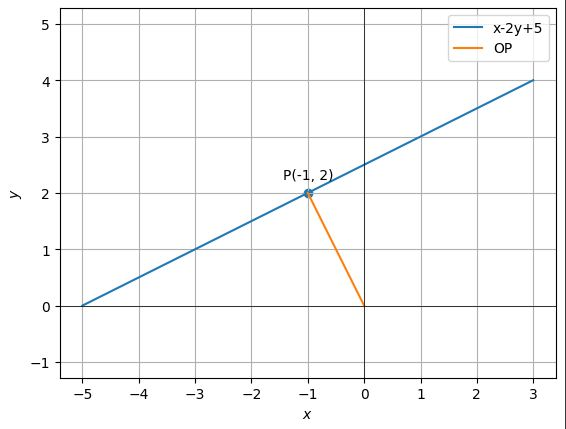
\includegraphics[width=\columnwidth]{figs/graph.jpg}
  \caption{Graph}
  \label{fig:pic}
\end{figure}
%\end{document}

\item $ABCD$ is a quadrilateral in which $AD = BC$ and $\angle{DAB} = \angle{CBA}$ as shown in figure \ref{fig:chapters/9/7/1/2/Fig}. Prove that
\begin{enumerate}
\item $\triangle{ABD} \cong \triangle{BAC}$
  \item $BD = AC$
  \item $\angle{ABD} = \angle{BAC}$
\end{enumerate}
	\solution
%\documentclass[12pt]{article}
%\usepackage[none]{hyphenat}
%\usepackage{amsmath}
%\usepackage{float}
%\usepackage{amssymb}
%\usepackage{graphicx}
%\usepackage{atbegshi}
%\AtBeginDocument{\AtBeginShipoutNext{\AtBeginShipoutDiscard}}
%\newcommand{\solution}{\noindent \textbf{Solution: }}
%\providecommand{\brak}[1]{\ensuremath{\left(#1\right)}}
%\newcommand{\myvec}[1]{\ensuremath{\begin{pmatrix}#1\end{pmatrix}}}
%\let\vec\mathbf
%\begin{document}
%\graphicspath{{./Documents}{./figs}}
%\begin{center}
%  \title{\textbf{Linear Forms}}
%  \date{\vspace{-5ex}}
%  \maketitle
%\end{center}
%\setcounter{page}{1}
%\section*{11$ ^{th} $ Maths - Chapter 10}
%The following problem is question 15 from exercise 10.3:
%\begin{enumerate}
%\item The perpendicular from the origin to the line $y=mx+c$ meets it at the point $(-1,2)$. Find the values of m and c.
%\end{enumerate}
%\solution \\
Given ,\\
the line line equation is

\begin{align}
   y&=mx+c
 \label{eq:1}
 \end{align}
\begin{align}
  \vec{P}&=\myvec{-1\\ \\2}\\
 \vec{O} &=\myvec{0\\ \\ 0}
\end{align}
   Direction Vector from $\vec{O}$ to point $\vec{P}$ is given by
    \begin{align}
    \vec{O - P} =\myvec{1\\ \\ -2}
 \end{align}
 If the lines are perpendicular then,
 \begin{align}
   \vec{(O - P)}^{\top}\vec{m} &= 0\\
   \myvec{1 & -2}\myvec{1 \\ \\ m}&=0\\
   1 - 2m &= 0\\
   m &= \frac{1}{2}
\end{align}
By substituting the m value in \eqref{eq:1},  we get
 \begin{align}
 2 &=\frac{1}{2} (-1) + c \\
 c &=\frac{5}{2}  
\end{align}
therefore,  Values of m and c are $\frac{1}{2}$ and $\frac{5}{2}$ \\
\begin{figure}[H]
  \centering
  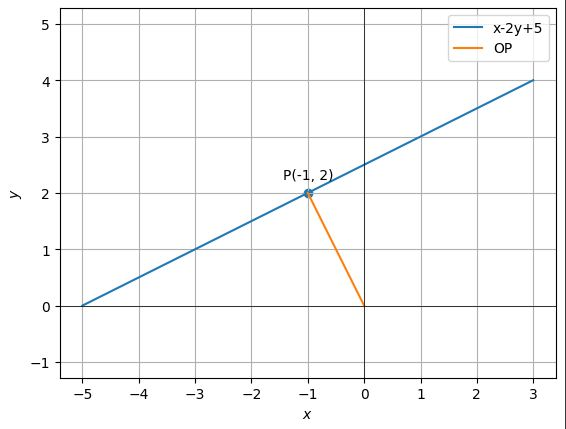
\includegraphics[width=\columnwidth]{figs/graph.jpg}
  \caption{Graph}
  \label{fig:pic}
\end{figure}
%\end{document}

\item $AD$ and $BC$ are equal perpendiculars to a line segment $AB$. Show that $CD$ bisects $AB$.\\
	\solution
%\documentclass[12pt]{article}
%\usepackage[none]{hyphenat}
%\usepackage{amsmath}
%\usepackage{float}
%\usepackage{amssymb}
%\usepackage{graphicx}
%\usepackage{atbegshi}
%\AtBeginDocument{\AtBeginShipoutNext{\AtBeginShipoutDiscard}}
%\newcommand{\solution}{\noindent \textbf{Solution: }}
%\providecommand{\brak}[1]{\ensuremath{\left(#1\right)}}
%\newcommand{\myvec}[1]{\ensuremath{\begin{pmatrix}#1\end{pmatrix}}}
%\let\vec\mathbf
%\begin{document}
%\graphicspath{{./Documents}{./figs}}
%\begin{center}
%  \title{\textbf{Linear Forms}}
%  \date{\vspace{-5ex}}
%  \maketitle
%\end{center}
%\setcounter{page}{1}
%\section*{11$ ^{th} $ Maths - Chapter 10}
%The following problem is question 15 from exercise 10.3:
%\begin{enumerate}
%\item The perpendicular from the origin to the line $y=mx+c$ meets it at the point $(-1,2)$. Find the values of m and c.
%\end{enumerate}
%\solution \\
Given ,\\
the line line equation is

\begin{align}
   y&=mx+c
 \label{eq:1}
 \end{align}
\begin{align}
  \vec{P}&=\myvec{-1\\ \\2}\\
 \vec{O} &=\myvec{0\\ \\ 0}
\end{align}
   Direction Vector from $\vec{O}$ to point $\vec{P}$ is given by
    \begin{align}
    \vec{O - P} =\myvec{1\\ \\ -2}
 \end{align}
 If the lines are perpendicular then,
 \begin{align}
   \vec{(O - P)}^{\top}\vec{m} &= 0\\
   \myvec{1 & -2}\myvec{1 \\ \\ m}&=0\\
   1 - 2m &= 0\\
   m &= \frac{1}{2}
\end{align}
By substituting the m value in \eqref{eq:1},  we get
 \begin{align}
 2 &=\frac{1}{2} (-1) + c \\
 c &=\frac{5}{2}  
\end{align}
therefore,  Values of m and c are $\frac{1}{2}$ and $\frac{5}{2}$ \\
\begin{figure}[H]
  \centering
  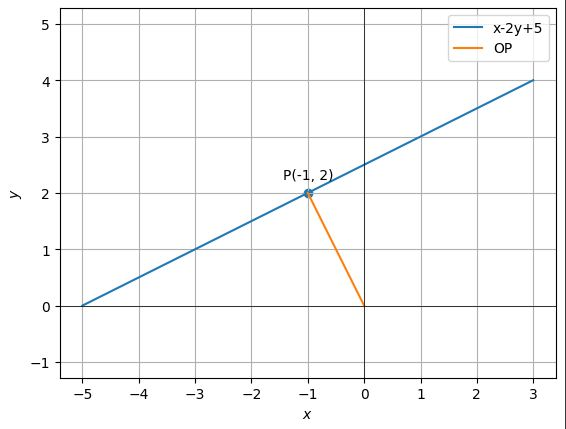
\includegraphics[width=\columnwidth]{figs/graph.jpg}
  \caption{Graph}
  \label{fig:pic}
\end{figure}
%\end{document}

\item
$l$ and $m$ are two parallel lines intersected by another pair of parallel lines $p$ and $q (\figref{fig:9.7.1.4})$,show that $\triangle ABC \cong \triangle CDA$.

\textbf{Figure :}
\begin{figure}[H]
    \centering
	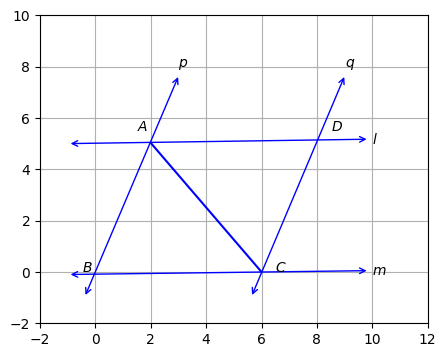
\includegraphics[width=\columnwidth]{chapters/9/7/1/4/fig/em1.png}
    \caption{Required parallelogram}
    \label{fig:9.7.1.4}
\end{figure}

\textbf{Solution :}
\begin{table}[H]
    \centering
      \begin{tabular}{|c|c|c|}
    \hline
        \textbf{Symbol} &\textbf{Description}&\textbf{Value}  \\
        \hline
        $\vec{B}$&Vertex at origin&$\vec{0}$\\
        \hline
        $a$ & Side of the parallelogram,$BC=DA$ & 6\\
        \hline
        $b$ & Side of the parallelogram,$AB=CD$& $\sqrt{29}$\\
        \hline
        $\theta$ & Angle of the parallelogram, $\angle ABC$& $\sin^{-1}\brak{{\frac{5}{\sqrt{29}}}}$\\
        \hline
    \end{tabular}

    \caption{Table of input parameters}
    \label{tab:9.7.1.4.1}
\end{table}

\begin{table}[H]
    \centering
       \begin{tabular}{|c|c|c|}
    \hline
        \textbf{Symbol} &\textbf{Description}&\textbf{Value}  \\
        \hline
	   $\vec{C}$&Vertex of parallelogram &$a\vec{e_1}$\\
        \hline
         $\vec{A}$&Vertex of parallelogram &$b\begin{pmatrix}
             \cos{\theta}\\
             \sin{\theta}
         \end{pmatrix}$\\
        \hline
        $\vec{D}$&Vertex of parallelogram &$\vec{C+A}$\\
        \hline
    \end{tabular}

    \caption{Table of output parameters}
    \label{tab:9.7.1.4.2}
\end{table}  
So,$\triangle ABC \cong \triangle CDA.\brak{by A-A-S}\brak{proved}$

\end{enumerate}
